\documentclass[9pt, conference]{IEEEtran}
\usepackage{url}
\usepackage{graphicx}
\usepackage{sidecap}
\usepackage{float}
\usepackage{wrapfig}
\usepackage{amsmath}

\title{COMP5411 Rendering Project Proposal: Rendering Thin Film Interference on Soap Bubbles}
\author{\IEEEauthorblockA{Mucong DING, 20323458\\mcding@connect.ust.hk\\Hong Kong University of Science and Technology}}

\begin{document}
\maketitle
\begin{abstract}
The computer graphics simulation of real-world optical effects is of great interest. In this project, I focus on the thin film interference of soap bubbles. Soap bubbles have fascinating optical properties which are difficult to be simulated by simple shading algorithm. Although generally, a shader which takes reflection, refraction and Fresnel effect into considerations can already produces acceptable results\cite{bubblebase}, there are many other interesting effects which are omitted. Among them, the dominant one is the thin film interference. Since the thickness of soap bubble film is around hundreds nanometers, thin film interference greatly affect the appearance of a soap bubble. In this proposal, we introduce a formula of the thin film reflectance $R(\theta, \lambda, d)$ which not only depends on incident angle $\theta$, but also varies with wave length $\lambda$ and thin film thickness $d$. Base on that, we can implement a shader which also handles interference effects, using \textit{webgl} and \textit{three.js}. Moreover, we propose some approaches to approximate the dynamics of bubble thickness $d$, especially for the draining and sloshing effects. This makes the interference effect more obvious to see and more lifelike.
\end{abstract}

\section{\label{sec1}A Skeleton Example}
\textit{three.js} provide a very simple example which use a self defined shader to render soap bubbles \cite{bubblebase}. As we can see from the Fig. \ref{bubbelbase}, that this shader use slightly different dynamic texture mappings to approximate the spectral splitting effects due to refraction. 

\begin{wrapfigure}{r}{0.7\linewidth}
	\vspace{-7pt}
	\centering
	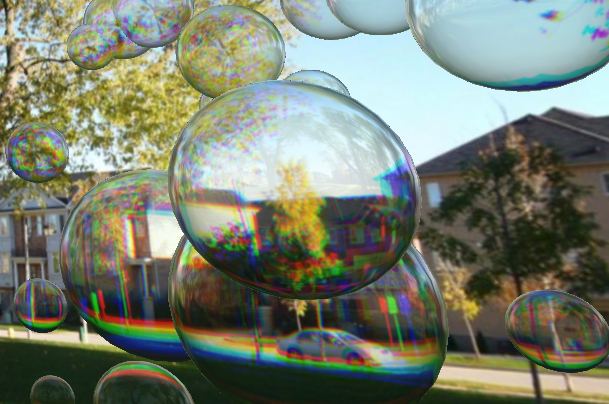
\includegraphics[width=0.7\linewidth]{bubble_base.png}
	\vspace{-10pt}
	\caption{\label{bubbelbase}Soap bubble Demo Example\cite{bubblebase}}
	\vspace{-7pt}
\end{wrapfigure}

Although this dynamic texturing already makes those spheres look like bubbles, it is very inadequate and not lifelike. Apart from the fact that it does not simulate real reflection and refraction with Fresnel effect, it mistakes the origin of "spectral texture" on the bubble surface. In general, since the thickness of bubble is not larger than 1 micrometer, the dominant effect of refraction is only a small displacement. The real cause of "spectral texture" is the thin film interference.

\section{\label{sec2}Thin Film Interference}
A complete model which simulate interference must takes the wave length $\lambda$ and thickness $d$ as parameters. In general, the radiance at point $P$ still consists of the transmitted and reflected components, as follows,
\begin{equation}
	L_P(\lambda) = (1-R(\lambda, \theta, d))L_{it}(\lambda) + R(\lambda, \theta, d)L_{ir}(\lambda)
\end{equation}
But the formula of reflectance look more complex \cite{interferencepaper},
\begin{equation}
\begin{split}
	R(\lambda, \theta, d) =& 2R_\bot^2\frac{1-\cos\delta}{1+R_\bot^4-2R_\bot^2\cos\delta}\\ &+2R_\parallel^2\frac{1-\cos\delta}{1+R_\parallel^4-2R_\parallel^2\cos\delta}
\end{split}
\end{equation}
Where $\delta$ is also a function of $\lambda$, $\theta$ and $d$,
\begin{equation}
	\delta(\lambda, \theta, d) = \frac{4\pi}{\lambda}nd\cos\theta
\end{equation}
With these equations, we are able to render the complete refraction, reflection and interference effects.

\section{\label{sec3}Dynamics of Thickness $d$}
In order to make the interference effect more obvious and lifelike, we should also consider the non-uniform distribution and dynamics of thickness $d$ on the bubble surface. In general, two dominant effects should be considered.

\begin{wrapfigure}{r}{0.5\linewidth}
	\vspace{-15pt}
	\centering
	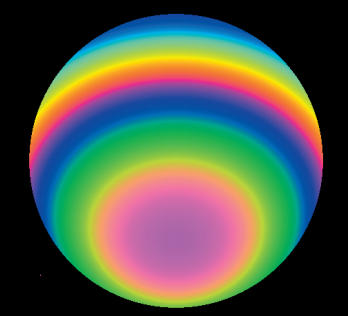
\includegraphics[width=0.5\linewidth]{thickness_gradient.png}
	\vspace{-10pt}
	\caption{\label{thicknessgradient}Thickness gradient \cite{888023}}
	\vspace{5pt}
	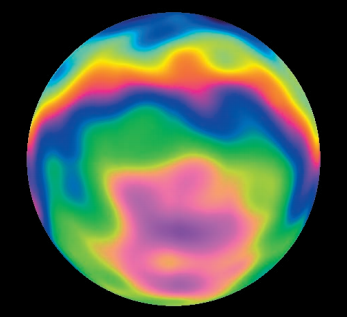
\includegraphics[width=0.5\linewidth]{thickness_sloshing.png}
	\vspace{-10pt}
	\caption{\label{thicknesssloaching}Thickness sloshing \cite{888023}}
	\vspace{-10pt}
\end{wrapfigure}
The first one is the vertical gradient of thickness due to draining and earth gravity. This makes the thickness distribution look like Fig. \ref{thicknessgradient}.

The second one is due to the perturbation of the environment around, there are random sloshing on the surface. When taking this into considerations, the thickness distribution is more like Fig. \ref{thicknesssloaching}.

\section{Objective and Expected Results}
\begin{wrapfigure}{r}{0.6\linewidth}
	\vspace{-7pt}
	\centering
	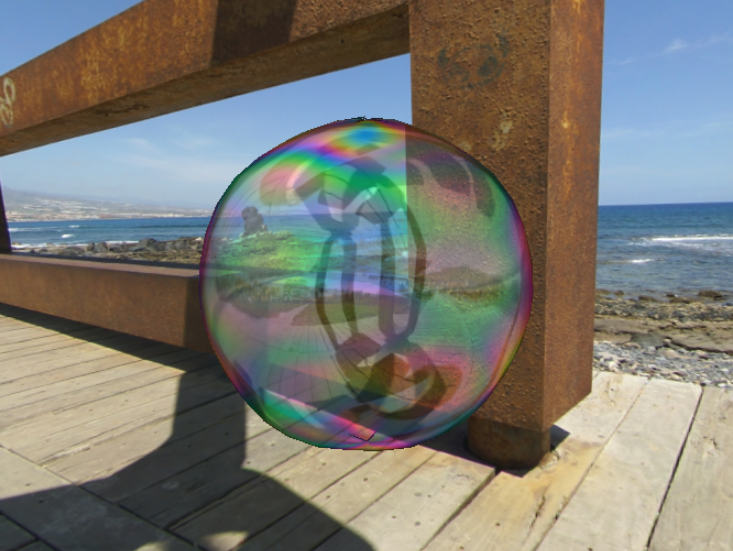
\includegraphics[width=0.6\linewidth]{bubble_expected.png}
	\vspace{-10pt}
	\caption{\label{bubbleexpected}Expected rendering results \cite{bubblebase}}
	\vspace{-7pt}
\end{wrapfigure}

The main objective is to extend the shader in the skeleton example described in Sec. \ref{sec1} using the radiance formula described in Sec. \ref{sec2} and also simulate the distribution and dynamics of thickness $d$ on the bubble surface according to Sec. \ref{sec3}. The original shader will be completed changed to implement the ideas described in this proposal, while the rest parts, which make extensive use of \textit{three.js} library, will remain the same.

The expected rendering result should exhibits lifelike interference textures on the surface, similar to the Fig. \ref{bubbleexpected}. I hope that we can optimize the algorithm and still achieve real-time rendering as in the original example. However, it is likely that we have to the number of bubbles in the scene to speed up the rendering. 


\bibliographystyle{IEEEtran}
\bibliography{reference}


\end{document}
